% filepath: report/3-result.tex
\section{Experiments}
We evaluate our agents via head-to-head matches under varying rule parameters. Below, we describe the experimental setup and present the resulting win-rate heatmaps. In all of our experiments, the board size is 8 and there are two players. 

\subsection{Experiment Setup}
In our tests, there are three key parameters:
\begin{itemize}
  \item Agent types: All possible pairings of the six agents.
  \item Maximum turns: 500.  
    If a match exceeds 500 steps, terminate and declare the player with more pawns in their goal area the winner.
  \item Total rounds: 100.  
    After 100 matches per pair, calculate each agent's win rate. we conducted only 50 matches due to its higher computational cost.
\end{itemize}

\subsection{Winning Condition}
A player is declared the winner in a single match based on the following rules:
\begin{itemize}
  \item We declare a winner immediately if one player has moved all the pawns into the goal area.  
  \item If 500 turns elapse without this condition, the player with more pawns in their goal area wins; if tied, the match is a draw.
\end{itemize}

\subsection{Experiment Results}
Under the above settings and winning conditions, we conducted head-to-head matches for every possible pairing of player types. The outcomes of these matches are summarized and visualized using heatmaps to highlight win rates and performance differences across agents.

The results are illustrated in Figure~\ref{fig:heatmap}, where each cell indicates the win rate (in percentage) of the first player (Sente, row) when playing against the second player (Gote, column). A higher value indicates a stronger performance of the row agent when moving first. The color gradient reflects the win rate, ranging from green (low) to red (high).

Note that win rates exclude drawn games and may therefore be non-integral values.

For clarity, the agents are abbreviated as follows. G (Greedy), M (Minimax), MLS (Minimax Local Search), MCTS (Monte Carlo Tree Search), AQL (Approximate Q-Learning), and NAQL (Neural Approximate Q-Learning).

\begin{figure}[h]
    \centering
    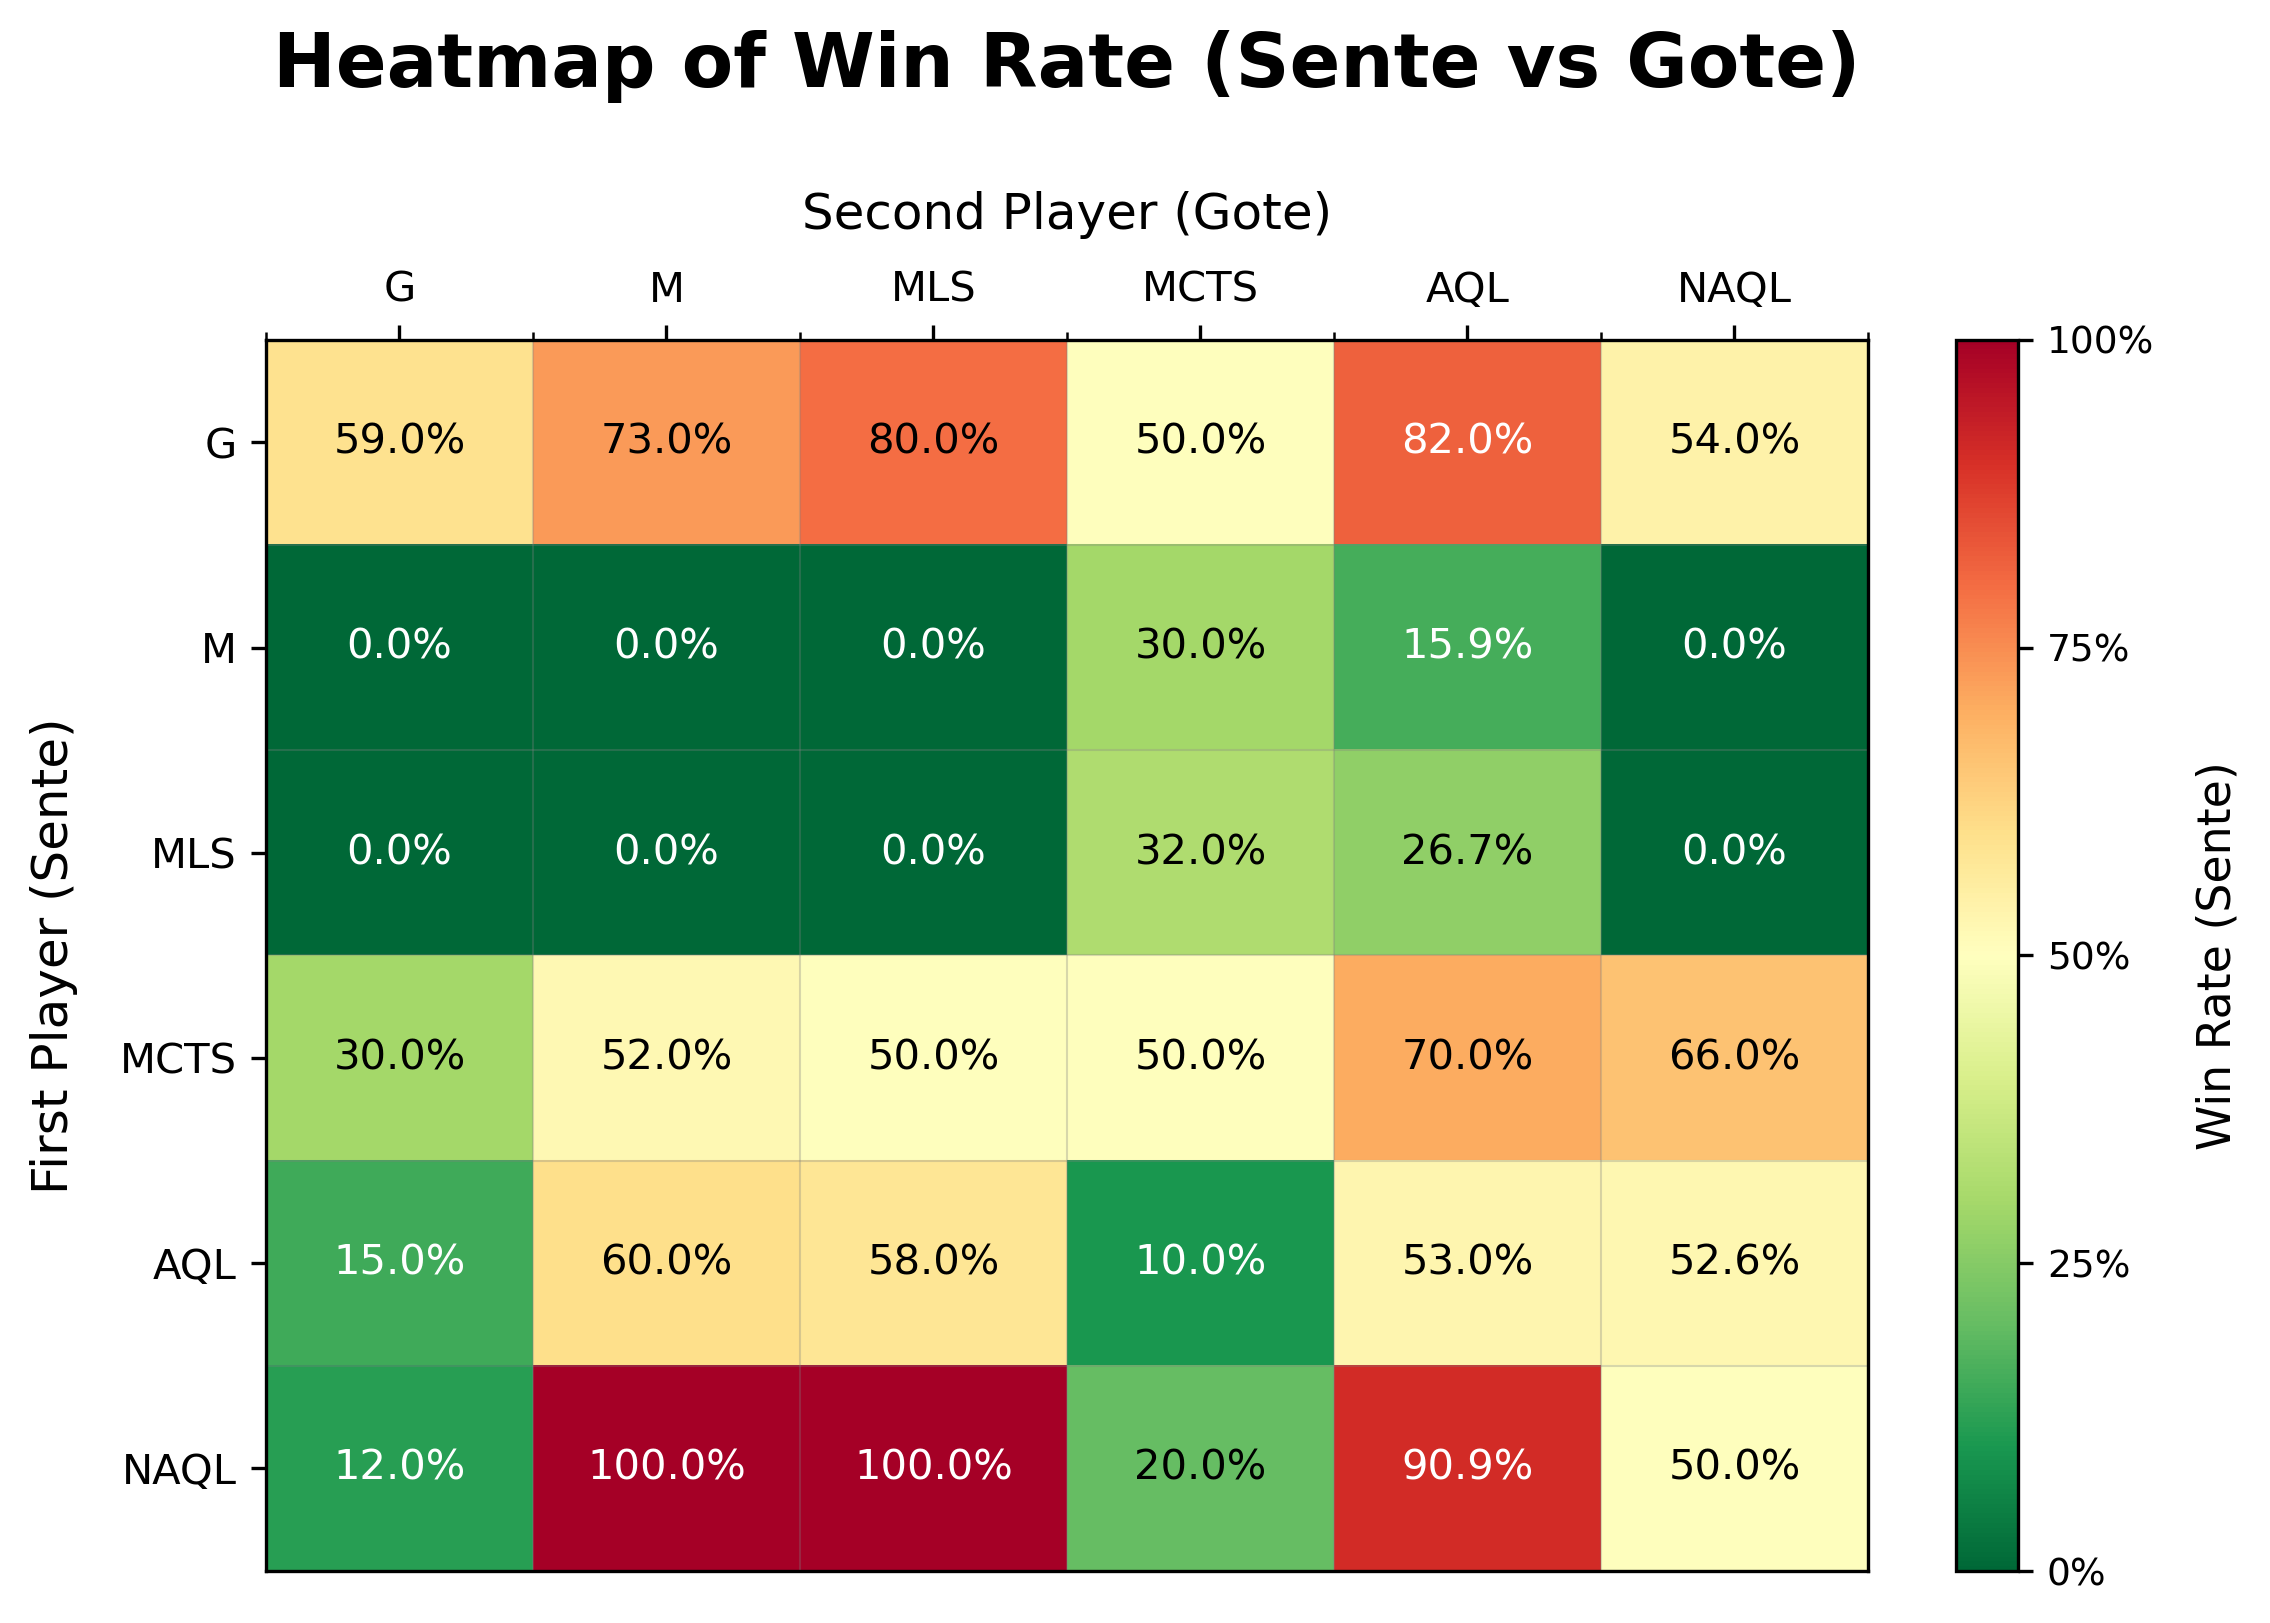
\includegraphics[width=1\columnwidth]{figures/win_rate_heatmap.png}
    \caption{Heatmap of Win Rate}
    \label{fig:heatmap}
\end{figure}